\section{Diagrama de Objetivos}

\subsection{Criterios preliminares}

A la hora de encarar un problema como el siguiente es importante identificar subproblemas que 
nos permitan construir de manera más simple una solución al mismo. En este caso identificamos que 
el problema de una elección puede dividirse temporalmente en tres etapas claras:

\begin{enumerate}
\item El proceso de preparación anterior al día de las elecciones.
\item El día de las elecciones.
\item El conteo de los votos emitidos.
\end{enumerate}

Se puede entonces decir que para lograr una elección exitosa necesitamos que estas tres etapas lo sean.\\

Este criterio será la base para la construcción del Diagrama de objetivos que modela los requerimientos necesarios del software.	\\

A continuación presentaremos el diagrama de objetivos del problema acompañado de un conjunto de escenarios descriptos de manera informal que ayudan a comprender el mismo.\\

A su vez consideramos la siguientes hipótesis de dominio:

\begin{itemize}
\item Todas las escuelas tienen conexión telefónica.
\item \textcolor{red}{Ponemos algo de las computadoras en red para el o-refinamiento?}
\end{itemize}

\newpage
\subsection{Diagrama}

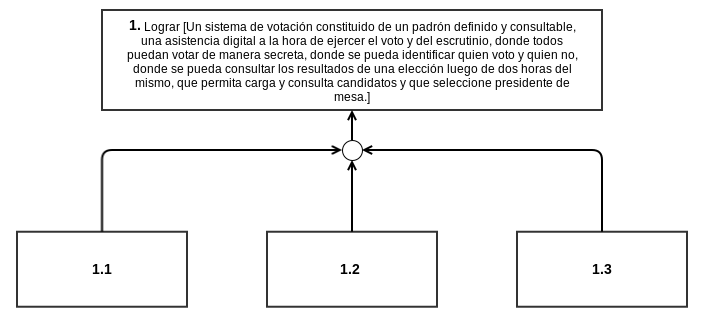
\includegraphics[scale=0.55]{imagenes/Diagramas/1.png}